%!TEX root = ../report.tex

\section{Design Patterns}
Design patterns are generalizations of detailed design knowledge from existing systems.
They provide a shared vocabulary and examples of reusable designs to designers (e.g. polymorphism, delegation/aggregation).

In summary, there are three types of design pattern:
\begin{itemize}
	\item \textbf{Structural Patterns}
		\begin{itemize}
			\item Reduce coupling between two or more classes
			\item Introduce an abstract class to enable future extensions
			\item Encapsulate complex structures
		\end{itemize}
	\item \textbf{Behavioral Patterns}
		\begin{itemize}
			\item Allow a choice between algorithms and the assignment of responsibilities to objects (\glqq Who does what?\grqq)
			\item Simplify complex control flows that are difficult to follow at runtime
		\end{itemize}
	\item \textbf{Creational Patterns}
		\begin{itemize}
			\item Allow a simplified view from complex instantiation processes
			\item Make the system independent from the way its objects are created,
			composed and represented
		\end{itemize}
\end{itemize}

The following sections list some of the most relevant patterns of those categories.

\newpage
\subsection{Structural Patterns}
Structural patterns aim for less coupling between classes and easier extensibility by encapsulating complex structures.

\subsubsection{Adapter Pattern/Wrapper}
Connects incompatible components to for example
\begin{itemize}
  \item Reuse existing components
  \item Convert an interface to another interface (maybe needed by an API call)
\end{itemize}

\begin{figure}[h]
	\centering
	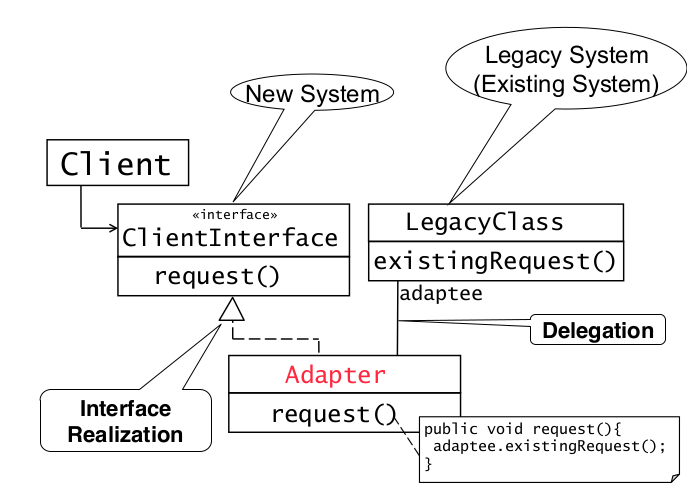
\includegraphics[width=\linewidth]{images/pattern_adapter.png}
	\caption{Structure of Adapter Pattern/Wrapper}
\end{figure}
\newpage

\subsubsection{Bridge Pattern}
Allows to delay the assignment of an implementation of an interface from compile to run time.
The \textbf{degenerated bridge pattern} is the same as the bridge pattern without the taxonomy in the application domain.

This pattern can be used to test the application with mocks e.g. a component is not yet implemented, so a mock is used to replace the component for testing purposes.

Another common use case is to provide support for multiple vendors of a specific service e.g. database vendors.

In contrast to the adapter pattern, the bridge pattern is used up-front in a design to let abstractions and implementations vary independently. 
\begin{figure}[h]
	\centering
	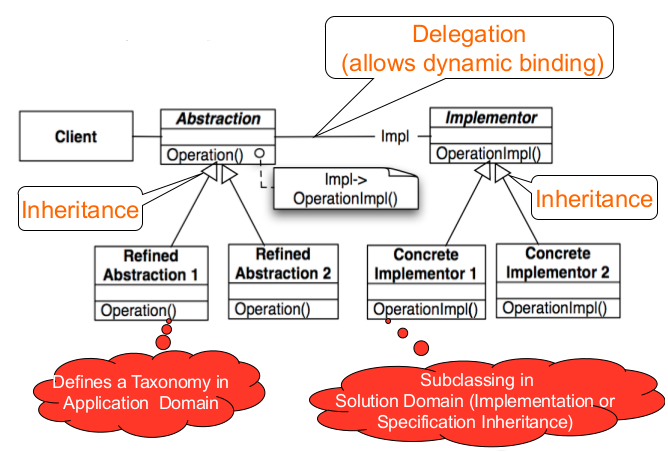
\includegraphics[width=\linewidth]{images/pattern_bridge.png}
	\caption{Structure of Adapter Pattern}
\end{figure}
\newpage

\subsubsection{Proxy Pattern/Caching}
The proxy pattern allows to defer object creation and object initialization to the time you need the object.

Some common use cases:
\begin{itemize}
	\item \textbf{Caching} (Remote Proxy)
		\subitem $\rightarrow$ Local object is representative for object in different address space
	\item \textbf{Substitute} (Virtual Proxy)
		\subitem $\rightarrow$ Object is expensive to create/download, proxy acts as stand-in
	\item \textbf{Access control} (Protection Proxy/Firewall)
		\subitem $\rightarrow$ Proxy object provides access control to the real object
\end{itemize}
\begin{figure}[h]
	\centering
	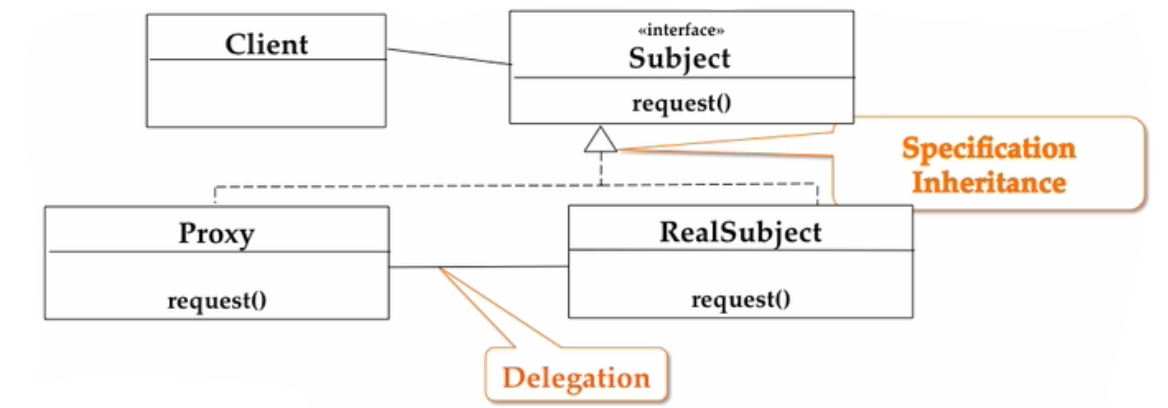
\includegraphics[width=\linewidth]{images/pattern_proxy.png}
	\caption{Structure of Proxy Pattern/Caching}{\textit{The client never calls \texttt{request()} in \texttt{RealSubject}, instead it always calls the method in \texttt{Proxy} which might delegate it to \texttt{RealSubject}.}}
\end{figure}
\newpage

\subsubsection{Composite Pattern}
The composite pattern models tree structures that represent part-whole hierarchies with arbitrary depth and width.
It lets the client treat individual objects and groups uniformly.
\begin{figure}[h]
	\centering
	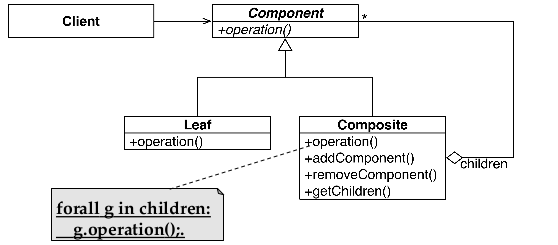
\includegraphics[width=\linewidth]{images/pattern_composite.png}
	\caption{Structure of Composite Pattern}
\end{figure}
\newpage


\subsection{Behavioral Patterns}
Behavioral patterns identify common communication patterns between objects and realize these patterns. By doing so, these patterns increase flexibility in carrying out this communication. %from wikipedia

\subsubsection{Strategy Pattern}
The strategy pattern is suited for situations where different algorithms are available for a problem (e.g. sorting).
In contrast to the bridge pattern, which is used for structural decisions, the strategy pattern choses the implementation to use at \textit{runtime} and therefore alters the behavior.
\begin{figure}[h]
	\centering
	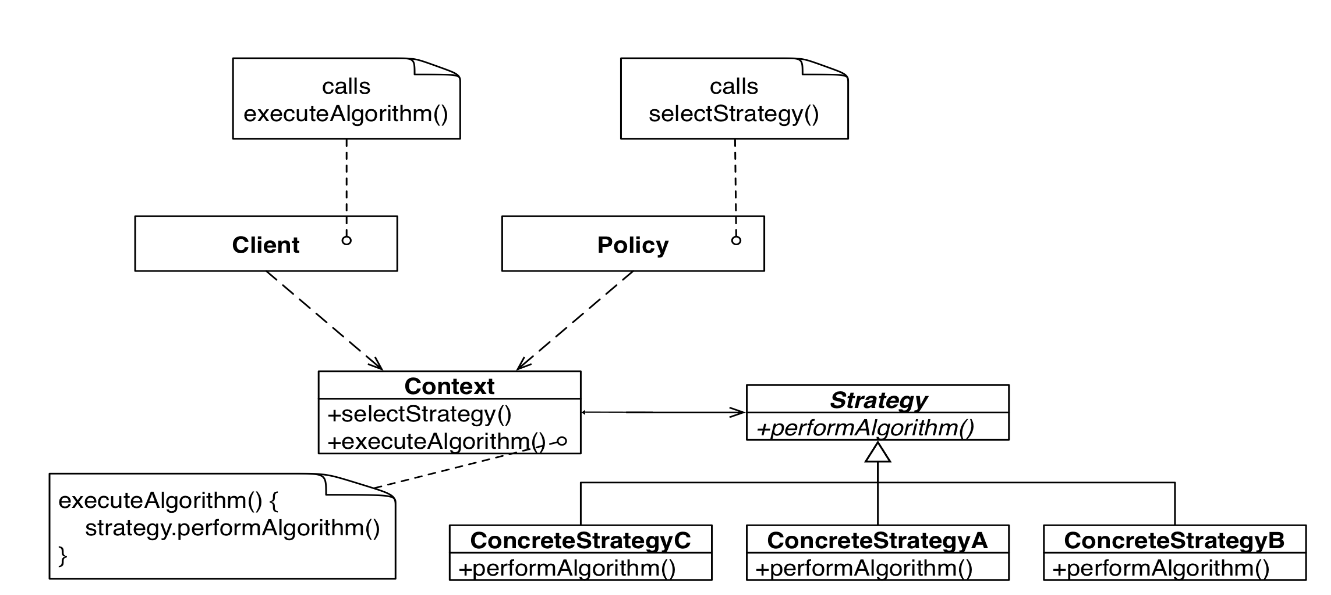
\includegraphics[width=\linewidth]{images/pattern_strategy.png}
	\caption{Structure of Strategy Pattern}{\textit{A strategy is chosen on \textbf{runtime} by the \texttt{Policy} class before the client calls \texttt{executeAlgorithm()}}}
\end{figure}
\newpage

\subsubsection{State Pattern}
Dependent on the current state of a system, an action should do different things (e.g. TCP open, close).
The state pattern avoids many if else statements and is flexible to add more cases/states.
Also the transitions between states are explicit.\newline

Problem: Where are state transactions handled?% (in the exercise of the lecture in the states)
\newline

In contrast to the strategy pattern, which handles different algorithms, the state pattern handles different states of an object.

\begin{figure}[h]
	\centering
	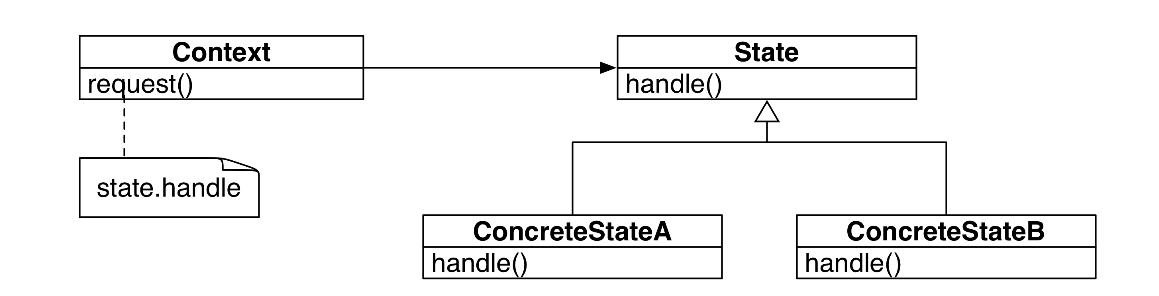
\includegraphics[width=\linewidth]{images/pattern_state.png}
	\caption{Structure of State Pattern}
\end{figure}
\newpage

\subsubsection{Observer Pattern}
The observer pattern handles changes in a publisher class and notifies all subscribers about that change (e.g. the user interface) to maintain consistency.
There are three variants for maintaining consistency:
\begin{itemize}
  \item \textbf{Push Notification:} Every time a state changes, all subscribers are notified
  \item \textbf{Push-Update Notification:} The publisher also sends the state that has changed
  \item \textbf{Pull Notification:} A subscriber inquiries about the state of the publisher
\end{itemize}

\begin{figure}[h]
	\centering
	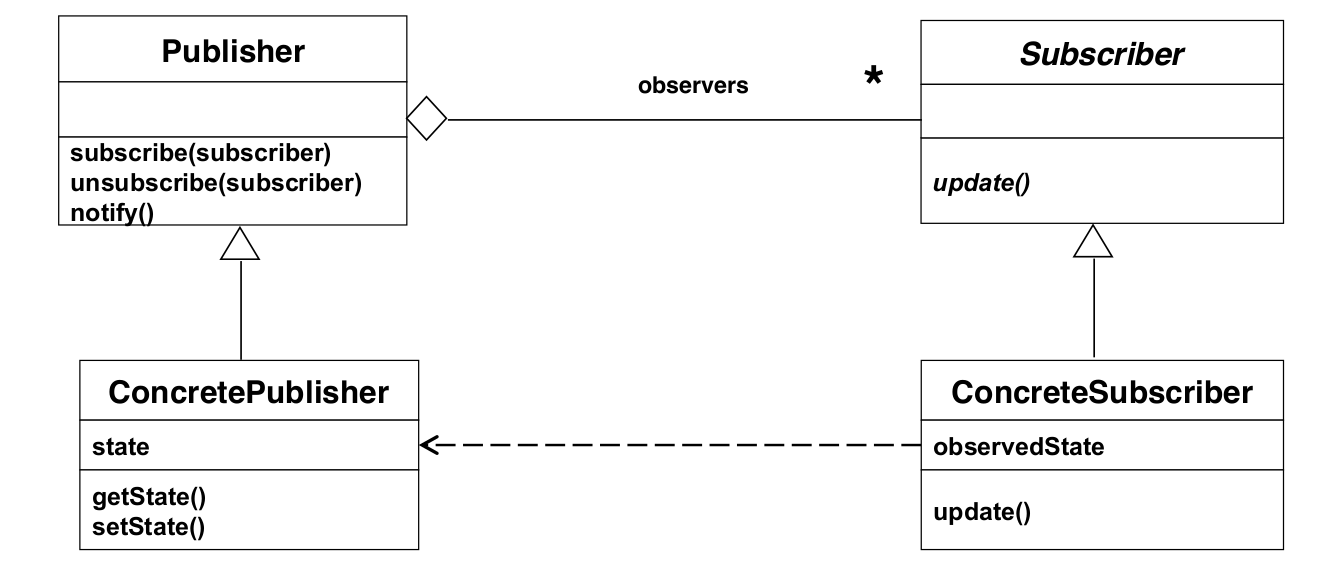
\includegraphics[width=\linewidth]{images/pattern_observer.png}
	\caption{Structure of Observer Pattern}
\end{figure}
\newpage

\subsubsection{Model View Controller Pattern}
The model-view-controller architectural style decouples data access and data representation.
The view handles the data representation, the model the data access and the controller handles the communication between the other two.\newline

In the \textbf{pull variant} the connection between the controller and the view is removed.
In this variant the view asks the model for the data explicitly.

In the \textbf{push notification variant} both the connection between the view and the model and controller respectively are removed.
When a change in the model occurs, the view and controller are updated via the observer pattern.

\begin{figure}[h]
	\centering
	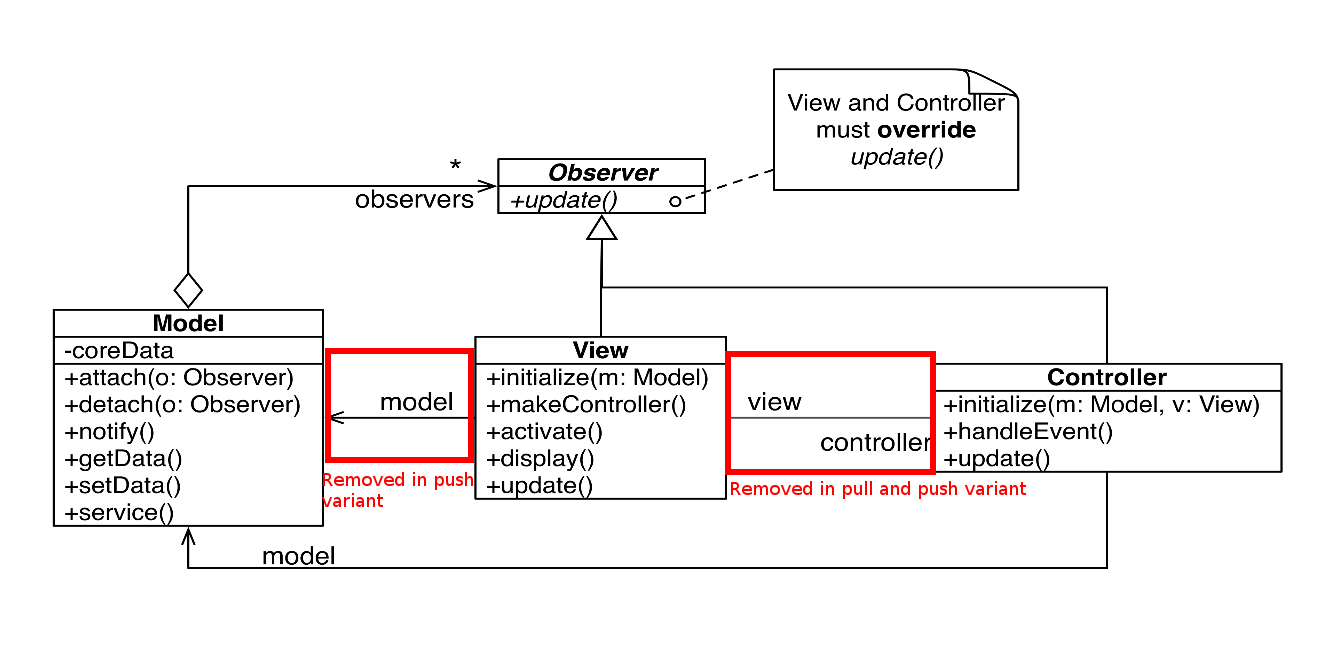
\includegraphics[width=\linewidth]{images/pattern_mvc.png}
	\caption{Structure of Model View Controller Pattern}
\end{figure}

\newpage

\subsubsection{Command Pattern}
The command pattern can be used to design user interfaces with multiple commands without using multiple \texttt{if}-statements (i.e. \texttt{if(command == x) {...} else if(command == y) ...}).
It can be used to make menus reusable across applications.
This reduces the complexity by decoupling boundary objects (e.g. menu buttons) from control objects (the concrete commands). Only these command objects can modify entity objects (the
Receivers).
When the user interface is changed, only the boundary objects need to be modified.\newline

Implementing Commands as classes allows command histories and thus \textit{undo} and \textit{redo} operations.\newline

\textbf{Common Applications:}
\begin{itemize}[topsep=5pt, itemsep=0pt]
  \item \textbf{Command Manager} Central repository for all commands
  \item \textbf{Redo/Undo Manager}
  \item \textbf{Queue} Holds commands until others objects are ready to do something with them
  \item \textbf{Dispatcher} (e.g. keyboard event loop)
\end{itemize}

\begin{figure}[h]
	\centering
	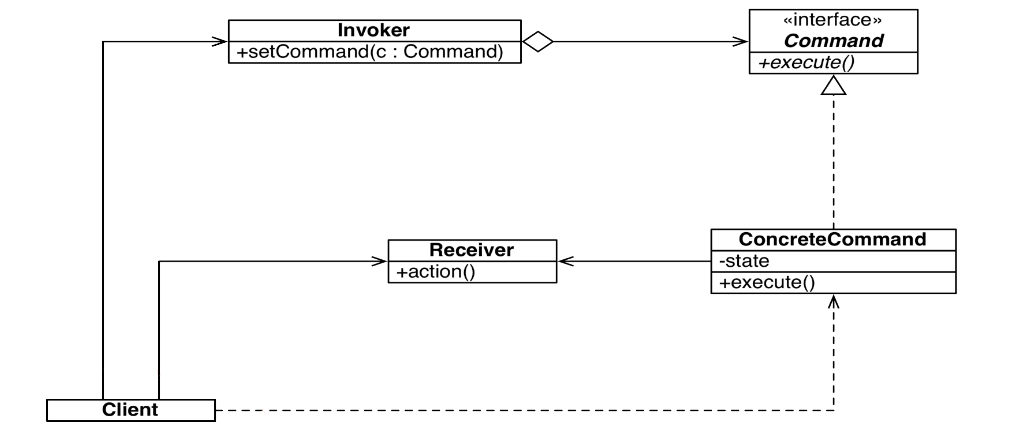
\includegraphics[width=\linewidth]{images/pattern_command.png}
	\caption{Structure of Command Pattern}
\end{figure}
\newpage


\subsection{Creational Patterns}
Creational patterns allow a simplified view from complex instantiation processes and make the system independent from the way its objects are created, composed and represented.

\subsubsection{Factory Pattern}
A factory class handles the instantiation of objects inheriting from one superclass depending on a keyword or value.
\begin{figure}[h]
	\centering
	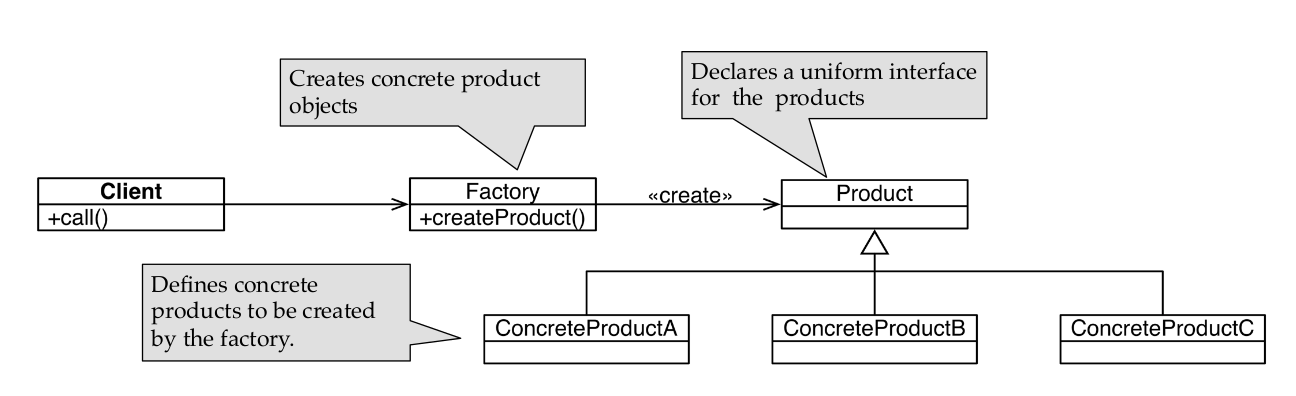
\includegraphics[width=\linewidth]{images/pattern_factory.png}
	\caption{Structure of Factory Pattern}
\end{figure}
\newpage

\subsubsection{Abstract Factory Pattern}
The abstract factory pattern is used to instantiate or initialize an object consisting of more subparts.
Every implementation of the abstract factory creates a set of components consisting of a variant of every part of the whole object.

\begin{figure}[h]
	\centering
	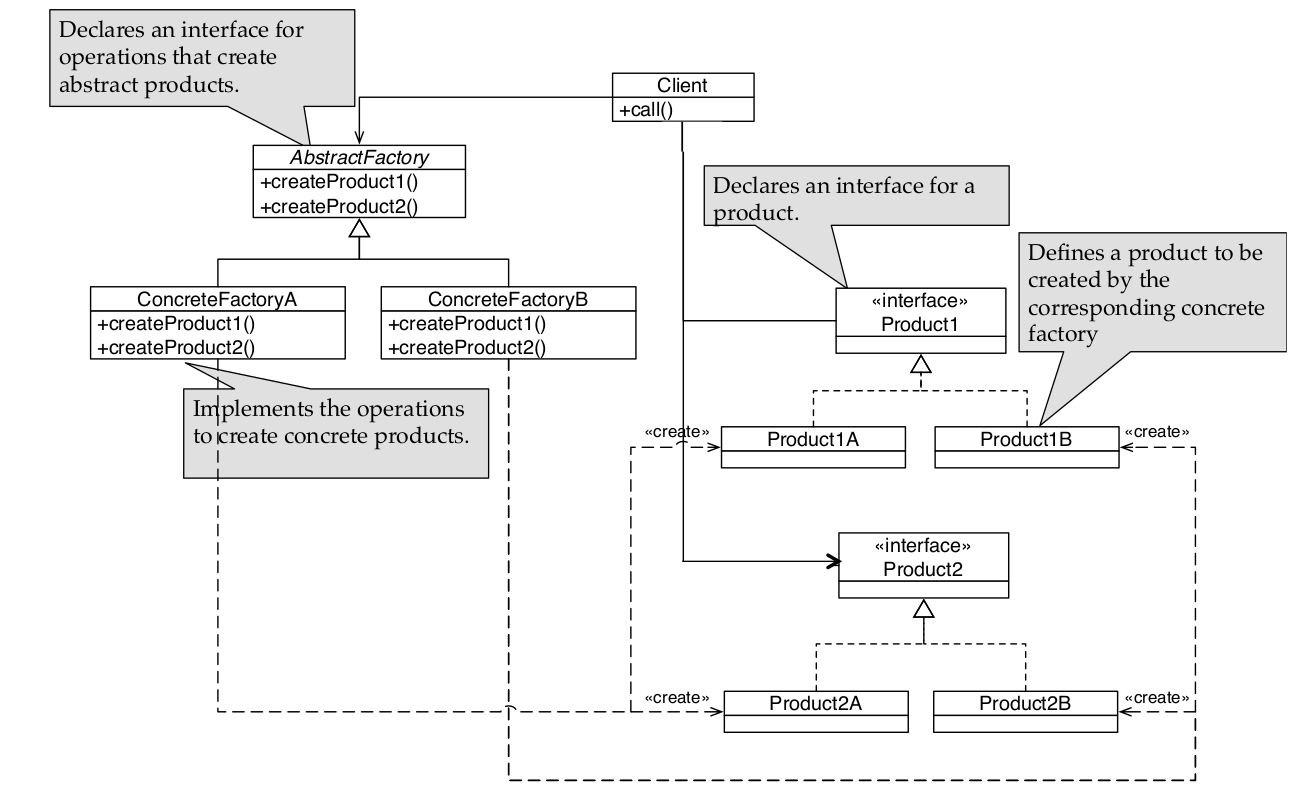
\includegraphics[width=\linewidth]{images/pattern_abstract_factory.png}
	\caption{Structure of Abstract Factory Pattern}
\end{figure}
\newpage


\subsection{Comparisons}

\subsubsection{Adapter vs. Bridge}
Both hide the detail of the underlying implementation, but:
\begin{itemize}
   \item the adapter (inheritance followed by delegation) is designed to handle incompatibilities
   \item the bridge (delegation followed by inheritance) is intended to differentiate between abstraction and implementation up-front
 \end{itemize}

 \subsubsection{Bridge vs. Strategy}
 The bridge is used for structural decisions on system startup whereas the strategy handles behavioral decisions on runtime based on changing criteria.

\subsubsection{Strategy vs. State}
The strategy pattern handles different algorithms at runtime whereas the state pattern handles different states of an object in the architecture.

\newpage
